% -----------------------------------------------------------------------------
% Resultados
% -----------------------------------------------------------------------------

\chapter{Result Analysis and Discussion - Sediment transport: Viscous Bedload}
\label{chap:Resultados-CFD}

    In this Chapter we will present the results obtained from the insertion of the fluid into the granular simulations. Our goal is to simulate the viscous bedload transport mode and extract the time transient $T_\textrm{sat}$ and the saturation length $L_\textrm{sat}$. The parameters we used to simulate the system is 10000 grains, with average diameter $d$ = 1 $\pm$ 20\%, with uniform distribution. Grains density $\rho^{g}$ = 6/$\pi$, leading the average mass $m$ = 1, the spring constant in the normal direction $k_{n}$ = 2500 and the spring constant in the tangential direction $k_{t}$ = 1875, the restitution coefficient $\epsilon \sim$ 0.25 (damping coefficient $\gamma \sim$ 42\% to the critical value), the friction coefficient $\mu$ = 0.5 between grain-grain contact. The bottom wall is made of fixed grains and has periodic boundary condition. The time step dt = $\frac{1}{50}\sqrt{\frac{m_r}{k_n}}$, the length $w$ = 1000$d$, the gravity acceleration $g$ = 1. The simulations are in a 2D dimensional space ($x,z$) but we use all parameters as if they are in 3D, and the third component $y$ has average width of 1$d$. Grains have spherical geometry. The fluid has the control parameters: density ratio between grains and fluid $\mathcal{D}_{R}$ = 2, Shields number varying from the range 0.05 $\leq$ $\Theta$ $\leq$ 0.5 equally spaced of $0.05$ units, and Galileo number varying from the range 0.01 $\leq$ $\mathcal{G}$ $\leq \sqrt{10}$ geometrically spaced of $\sqrt{10}$ units. Viscosity $\nu$ is controlled by Galileo number $\mathcal{G}$ (Equation \ref{equ:Reynolds}) and the characteristic imposed shear velocity $u_{*}$ is controlled by Shields number $\Theta$ (\ref{equ:Shields}). The preparation of the grains is done letting the grains fall by gravity, like a rain-like deposition, into the substrate, and after all grains fall, a controlled wind blows inside the grains, moving them into the direction we impose the future fluid profile. The fluid profile is then set to be zero layer by layer, allowing grains to rest, and in the end, the fluid has no motion. This eliminates any residual trace (preparation history) of the rain-like properties. Then the free grains are set to have a height of 10$d$ grains, and the grains below this 10$d$ column of free grains compounds the base wall. Then the fluid is imposed to have constant shear $\tau = \rho^f {u_{*}}^2$ at 10$d$ above the granular bed. We set the reference level 0$d$ at the granular bed, like in Figure \ref{fig:TM_profiles} $z$ axis. The fluid evolves from the top to the bed with the time constant as described in Equation \ref{equ:viscous_transient_velocity_full_solution} ($T = (\frac{4h^2}{\pi^2 \nu}$). We wait the fluid reaches the steady-state exchanging momentum with the grains and then we start to measure the profiles, like the ones presented in Figure \ref{fig:TM_profiles}. The steady-state is achieved when the total shear $\tau=\tau^f+\tau^p$ is constant.

\begin{figure}
    \centering
    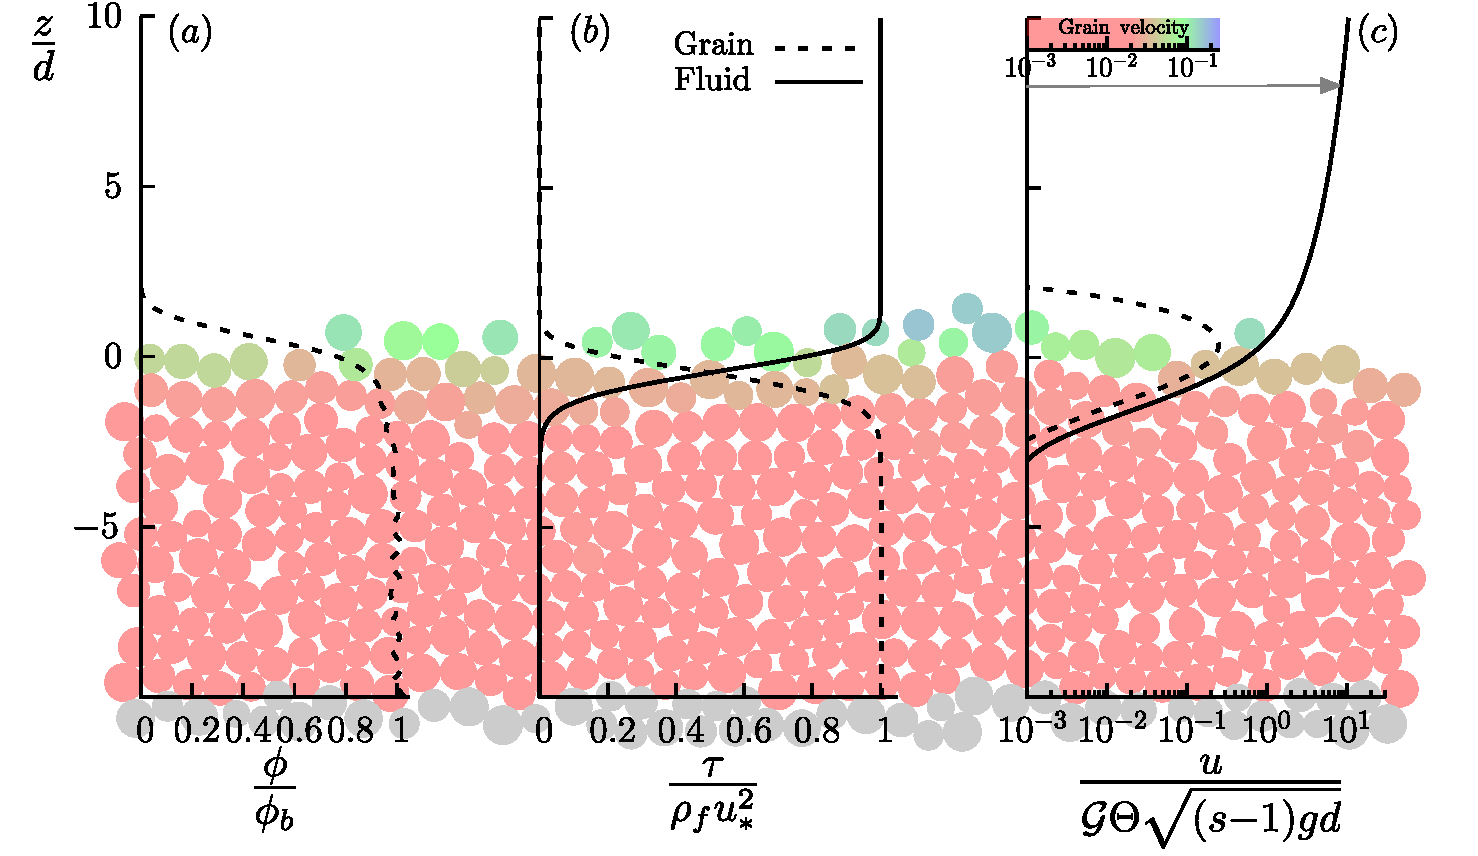
\includegraphics[width=0.9\linewidth]{04-figuras/TM-profiles.pdf}
    \caption[Transport profiles.]{Schematics of the numerical set-up, with typical vertical ($z$) profiles of packing fraction (a), shear stress (b) and velocity (c), here all computed with Galileo number $\mathcal{G}=0.3$ and Shields number $\Theta=0.3$ in the steady and homogenous case. The full system comprises about $10^4$ grains ($1000d$ in length) and has periodic boundary conditions in the horizontal ($x$) flow direction. (a) Volume fraction $\phi$ normalised by its value in the bulk of the bed $\phi_b$. (b) Shear stress carried by the fluid (solid line) and by the grains (dashed line), normalised by the stress $\rho_f u_*^2$ applied at the top of the fluid. (c) Normalised velocity of the fluid (solid line) and of the grains (dashed line). Flow is from left to right (arrow). On this snapshot, the colour of the grains codes for their instantaneous velocity (inset) -- grey grains are the fixed bottom plate.}
    \label{fig:TM_profiles}
\end{figure}

\section{Steady and homogeneous transport}
    We explore the steady-state by the transport laws described in the set of Equations \ref{equ:flux_steadystate_model} in Figure \ref{fig:TM_profiles}. To average the quantities we made three different starting samples and run long time simulations (10$T_\textrm{sat}$) in steady-state. The error bars are shown in figure, except if the associated error is smaller than the symbol.

\begin{figure}
    \centering
    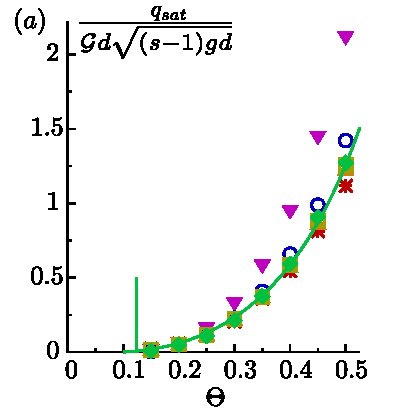
\includegraphics[width=0.495\linewidth]{04-figuras/TMa-qsat.pdf}
    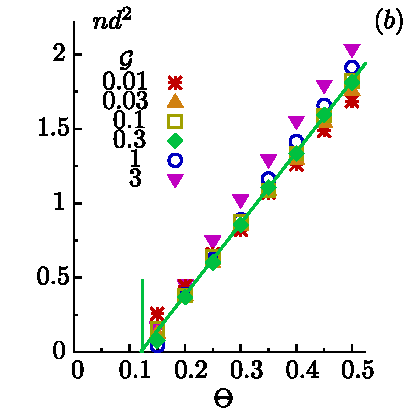
\includegraphics[width=0.495\linewidth]{04-figuras/TMb-nsat.pdf}
    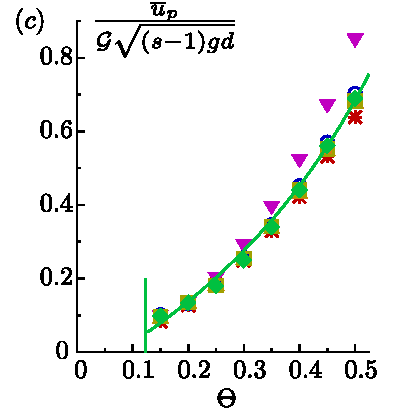
\includegraphics[width=0.495\linewidth]{04-figuras/TMc-usat.pdf}
    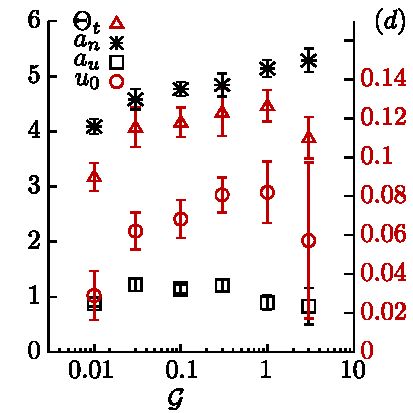
\includegraphics[width=0.495\linewidth]{04-figuras/TMd-adjustsat.pdf}
    \caption[Transport laws for viscous bedload transport.]{Transport laws as functions of $\Theta$ in the steady and homogenous case: saturated sediment flux $q_\textrm{sat}$ (a), moving grain density $n$ (b) and average grain velocity $\bar{u}_p$ (c), plotted in a normalised way to obtain a quasi data collapse. The symbols correspond to different values of $\mathcal{G}$ ranging from $0.01$ to $3$ (legend). Green solid curves: fit of the data following set of Equations \ref{equ:flux_steadystate_model}, for $\mathcal{G}=0.3$. Small vertical green line: visualisation of the Shield threshold $\Theta_t$, also for $\mathcal{G}=0.3$. Panel (d): variation of the fitting parameters with the Galileo number -- black (red) symbols associated with left (right) axis.}
    \label{fig:TM_profiles}
\end{figure}

\section{Temporal response and saturation time}
\label{sec:Tsat}
    From Equation \ref{equ:transporte}, with homogeneous wind in the $x$ direction, we simplify the equation, eliminating the factor $L_sat$ and any spatial variation for the flux, since $\partial q/\partial x = 0$. Then solving the differential equation, we expect to extract the saturation time $T_\textrm{sat}$ from the form:
\begin{equation}
    q(t) = q_\textrm{sat} + \delta q_\textrm{sat} e^{-t/T_\textrm{sat}}.
\end{equation}

    After completing the steady-state profiles, we instantly switch the entire fluid profile and measure the temporal transition of the grains to the new fluid profile. We chose to do this instant switch to have a small interference of the fluid, once the transition time for the fluid is related to the viscosity $\nu$ and the height $h$ of the imposed shear. The Figure \ref{fig:TM_transition} shows the time transient $T_\textrm{sat}$ for Galileo number $\mathcal{G}$ = 0.3 and the transition from Shields number $\Theta$ from 0.25 to 0.3 in Figure \ref{fig:TM_transition}(a) and the transition from $\Theta$ from 0.3 to 0.25 in Figure \ref{fig:TM_transition}(b).

\begin{figure}
    \centering
    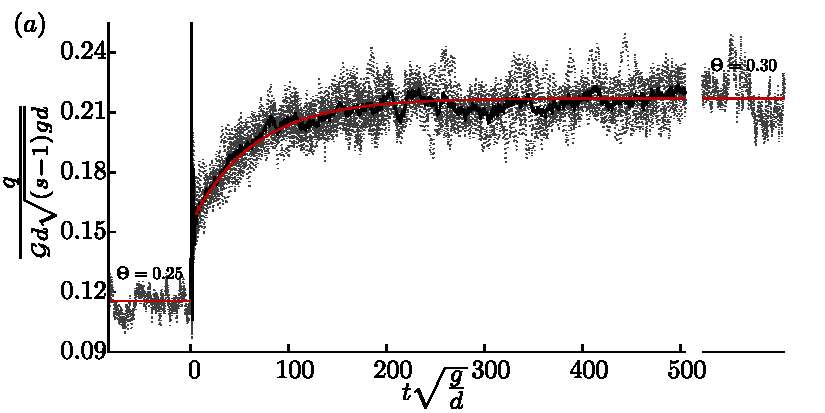
\includegraphics[width=0.8\linewidth]{04-figuras/TMa-transitionqup.pdf}
    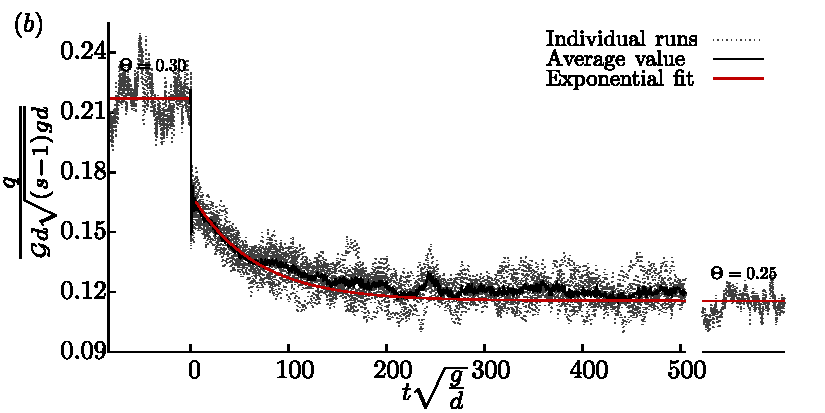
\includegraphics[width=0.8\linewidth]{04-figuras/TMb-transitionqdown.pdf}
    \caption[Temporal transport transition.]{Time transient of the sediment flux $q$ from one steady state to another, when the Shields number is suddenly increased (a) or decreased (b) by some small amount at $t=0$. The dash lines show individual runs and the solid lines their ensemble average (legend). Red line: exponential fit to extract the response saturation time, here $T^q_\textrm{sat}$. This example is for $\mathcal{G}=0.3$.}
    \label{fig:TM_transition}
\end{figure}

    Gathering the time transient $T_\textrm{sat}$ from different Shields number $\Theta$ for each Galileo number $\mathcal{G}$ we saw that the time transient $T_\textrm{sat}$ is invariant with Shields number $\Theta$ and inversely proportional to $\mathcal{G}$, as shown in Figrue \ref{fig:TM_tsat}(b). The limit of the viscous bedload regime is then expected to be until $\mathcal{G} \leq$ 1. Measuring the saturation time for $q$, $n$ and $\bar{u}_{p}$ are in same order of magnitude. Transitions below to the threshold $\Theta_t$ does not happen as grains does not move, while transitions near the threshold is very noisy, with huge errors associated to the measurement.

\begin{figure}
    \centering
    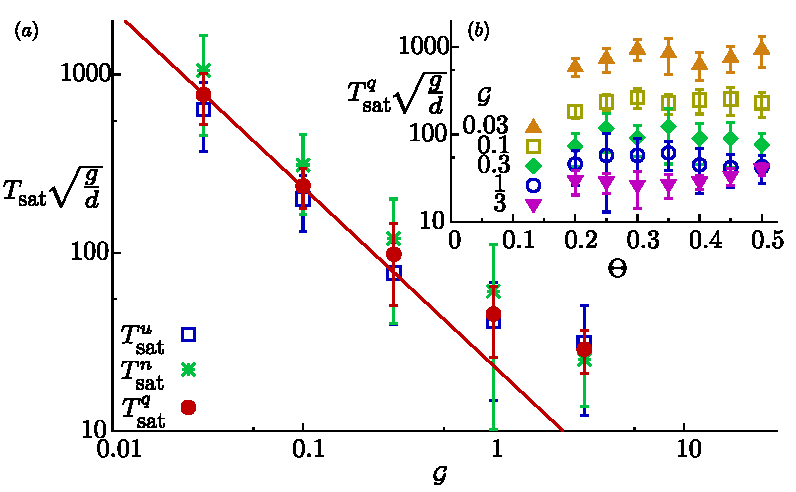
\includegraphics[width=0.75\linewidth]{04-figuras/TM-tRe.pdf}
    \caption[Saturation time $T_\textrm{sat}$ for the transport.]{Variation of the saturation time with the Galileo number. (a) Symbols: $T_\textrm{sat}$ associated with the time responses of $\bar{u}_p$, $n$ and $q$ (legend). Solide red line: inverse law $\propto 1/\mathcal{G}$ in this log-log representation. (b) Values of $T^q_\textrm{sat}$ for various $\Theta$.}
    \label{fig:TM_tsat}
\end{figure}

\section{Spatial perturbation and saturation length}
\label{sec:Lsat}
    To investigate the spatial relaxation of bedload transport, the idea is to consider a `sinusoidal wind' associated with a spatial modulation of the Shields number: $\Theta(x) = \Theta_0 + \delta\Theta \cos (kx)$. Assuming that $\delta\Theta \ll \Theta_0$, one can linearise the set of Equations \ref{equ:flux_steadystate_model} with respect to $\delta\Theta$ to obtain a modulated saturated flux:
%
\begin{equation}
q_\textrm{sat} = q_\textrm{sat}(\Theta_0) \left\{ 1 + \delta\Theta \left[ \frac{1}{\Theta_0 - \Theta_t} + \frac{1}{\Theta_0 - \Theta_t + u_0} + \frac{a_u}{1 - a_u \left( \Theta_0 - \Theta_t \right)} \right] \cos \left( kx \right) \right\},
\label{eq:modulated_saturatedflux}
\end{equation}
%
which is in phase with Shields number. Denoting by $\epsilon$ the factor of the cosine in the above expression, the linear response of the actual flux shall take the form
%
\begin{equation}
q = q_\textrm{sat}(\Theta_0) \left[ 1 + \zeta \epsilon \cos \left( kx - \varphi \right) \right].
\label{eq:modulated_flux}
\end{equation}
%
The relative amplitude $\zeta$ and the phase shift $\varphi$ are related to $T_\textrm{sat}$ and $L_\textrm{sat}$ through the relaxation equation (\ref{equ:transporte}), from which one obtains:
%
\begin{equation}
T_\textrm{sat} \frac{d\varphi}{dt} = - \frac{1}{\zeta} \sin\varphi + kL_\textrm{sat}
\qquad \mbox{and} \qquad
T_\textrm{sat} \frac{d\zeta}{dt} = - \zeta + \cos\varphi.
\label{eq:phase_and_amplitude_evolution}
\end{equation}
%
The integration of these equations give $\zeta(t)$ and $\varphi(t)$ that start linearly with time for $t \ll T_\textrm{sat}$, and then saturate to asymptotic values $\tan\varphi_\infty = kL_\textrm{sat}$ and $\zeta_\infty = \cos\varphi_\infty$ as soon as $t \gtrsim 2 T_\textrm{sat}$. Here we will use the measurement of those asymptotic values to deduce the saturation length $L_\textrm{sat}$.

    The way to induce this linearisation proposed to achieve the `sinusoidal wind' we turn off the feedback of the grains into the fluid, making the fluid profile fixed according to time, but modulated in the $x$ direction. The Figure \ref{fig:TM_lsat} shows the values of $L_\textrm{sat}$. Our main idea is to relate $L_\textrm{sat}$ with other parameters, mainly $T_\textrm{sat}$. We could extract the following prediction:
\begin{equation}
    L_\textrm{sat} \propto \bar{u}^p T_\textrm{sat},
\end{equation}
and the proportionality constant is about 3.7. With this prediction, we can simulate the system to be in quadrature of phase between the imposed wind and the flux response.

\begin{figure}
    \centering
    \parbox{0.495\textwidth}{
        \centering
        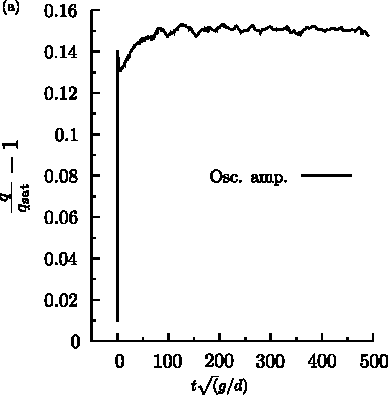
\includegraphics[width=0.495\textwidth]{04-figuras/TMa-qamp.pdf}
        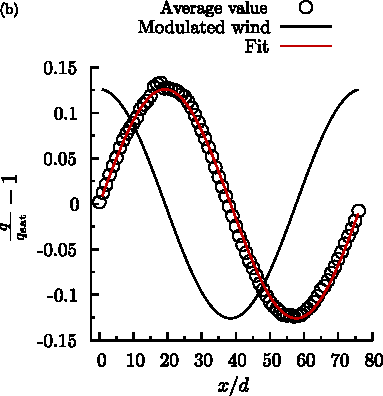
\includegraphics[width=0.495\textwidth]{04-figuras/TMb-qwind.pdf}
    }
    \parbox{0.495\textwidth}{
        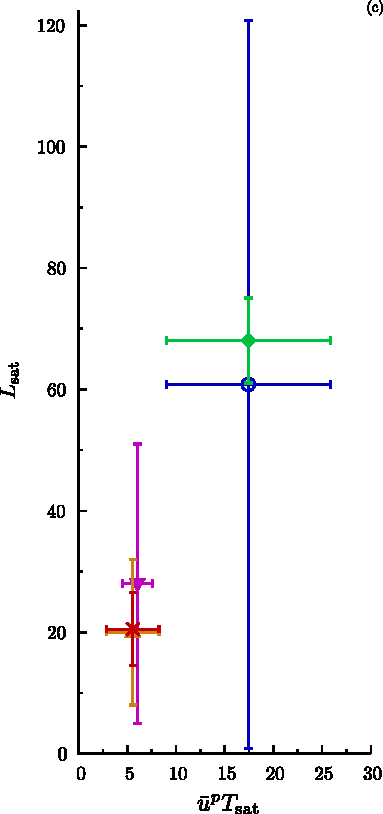
\includegraphics[width=0.495\textwidth]{04-figuras/TMc-Lsat.pdf}
    }
    \caption[Saturation length $L_\textrm{sat}$ for the transport.]{Example of modulated flux with the imposed wind (a). The amplitude of the modulated response in time: the amplitude takes about 2$T_\textrm{sat}$ to accommodate (a) and we extract the temporal cumulated response in (b). Finally, the saturation length is extracted from the difference of the curves imposed flux versus flux response (c). Each point in (c) corresponds to the curves with following parameters: \textcolor{red}{*} - $\mathcal{G}=0.3$ - $\Theta=0.25$ - $k=\frac{2\pi 13}{1000}$, \textcolor{orange}{$\blacksquare$} - $\mathcal{G}=0.3$ - $\Theta=0.25$ - $k=\frac{2\pi 5}{1000}$, \textcolor{magenta}{$\blacktriangledown$} - $\mathcal{G}=0.1$ - $\Theta=0.3$ - $k=\frac{2\pi 4}{1000}$, \textcolor{blue}{$\circ$} - $\mathcal{G}=0.3$ - $\Theta=0.45$ - $k=\frac{2\pi 13}{1000}$ and \textcolor{green}{$\Diamondblack$} - $\mathcal{G}=0.3$ - $\Theta=0.45$ - $k=\frac{2\pi 4}{1000}$. The more in quadrature the wind is, the less the error in extracting $L_\textrm{sat}$.}
    \label{fig:TM_lsat}
\end{figure}

%$\varphi(t) = a_\varphi t/T_\textrm{sat}$ and $\zeta(t) = a_\zeta t/T_\textrm{sat}$ for $t \ll T_\textrm{sat}$\\
%with $a_\varphi = kL_\textrm{sat}/2$ and $a_\zeta=1$

    Next Chapter we conclude this thesis, and set the open perspectives to continue this work.
